% !Rnw weave = knitr

\documentclass{article}\usepackage[]{graphicx}\usepackage[]{color}
%% maxwidth is the original width if it is less than linewidth
%% otherwise use linewidth (to make sure the graphics do not exceed the margin)
\makeatletter
\def\maxwidth{ %
  \ifdim\Gin@nat@width>\linewidth
    \linewidth
  \else
    \Gin@nat@width
  \fi
}
\makeatother

\definecolor{fgcolor}{rgb}{0.345, 0.345, 0.345}
\newcommand{\hlnum}[1]{\textcolor[rgb]{0.686,0.059,0.569}{#1}}%
\newcommand{\hlstr}[1]{\textcolor[rgb]{0.192,0.494,0.8}{#1}}%
\newcommand{\hlcom}[1]{\textcolor[rgb]{0.678,0.584,0.686}{\textit{#1}}}%
\newcommand{\hlopt}[1]{\textcolor[rgb]{0,0,0}{#1}}%
\newcommand{\hlstd}[1]{\textcolor[rgb]{0.345,0.345,0.345}{#1}}%
\newcommand{\hlkwa}[1]{\textcolor[rgb]{0.161,0.373,0.58}{\textbf{#1}}}%
\newcommand{\hlkwb}[1]{\textcolor[rgb]{0.69,0.353,0.396}{#1}}%
\newcommand{\hlkwc}[1]{\textcolor[rgb]{0.333,0.667,0.333}{#1}}%
\newcommand{\hlkwd}[1]{\textcolor[rgb]{0.737,0.353,0.396}{\textbf{#1}}}%
\let\hlipl\hlkwb

\usepackage{framed}
\makeatletter
\newenvironment{kframe}{%
 \def\at@end@of@kframe{}%
 \ifinner\ifhmode%
  \def\at@end@of@kframe{\end{minipage}}%
  \begin{minipage}{\columnwidth}%
 \fi\fi%
 \def\FrameCommand##1{\hskip\@totalleftmargin \hskip-\fboxsep
 \colorbox{shadecolor}{##1}\hskip-\fboxsep
     % There is no \\@totalrightmargin, so:
     \hskip-\linewidth \hskip-\@totalleftmargin \hskip\columnwidth}%
 \MakeFramed {\advance\hsize-\width
   \@totalleftmargin\z@ \linewidth\hsize
   \@setminipage}}%
 {\par\unskip\endMakeFramed%
 \at@end@of@kframe}
\makeatother

\definecolor{shadecolor}{rgb}{.97, .97, .97}
\definecolor{messagecolor}{rgb}{0, 0, 0}
\definecolor{warningcolor}{rgb}{1, 0, 1}
\definecolor{errorcolor}{rgb}{1, 0, 0}
\newenvironment{knitrout}{}{} % an empty environment to be redefined in TeX

\usepackage{alltt}

\usepackage{url}
\usepackage{underscore}

\title{Functional analysis of gene lists\\
\textbf{...WORK IN PROGRESS...}}
\author{Ferran Brians\'o and Alex S\'anchez-Pla. \\ Statistics department. UB \\ \& Statistics and Bioinformatics Unit (UEB). VHIR.}

\bibliographystyle{plain}
\IfFileExists{upquote.sty}{\usepackage{upquote}}{}
\begin{document}

\maketitle
\tableofcontents








\section{Introduction}

This document provides some information on the different analyses perfomed on several gene lists to help gain biological insight on the results of a differential expression analysis. Overall these analyses are known as \emph{Functional Analysis}.

Functional analysis can be performed in many different ways that lead to similar (or not-so-similar) results.  Because there is not a universal acceptance of what is a \texttt{complete, well done functional analysis} some different approaches will be shown and an arbitrary selection based on "doability", "scriptability" and of course "interpretability" will be performed.

Complementary information to this document can be found at \url{http://eib.stat.ub.edu/GO2016}

\subsection{Input Data for Functional Analysis}

Functional analysis can be made, on a first approach on
\begin{itemize}
\item A list of genes selected by being differentially expressed in a given experimental setting.
\item The whole list of genes -or even the whole expression matrix- that has been used in the analysis.
\end{itemize}

Most tools require that gene list consist of gene identifiers in some standard notation such as \texttt{Entrez}, \texttt{ENSEMBL} or other related to these.

These gene lists can be easily extracted from output tables provided by microarrays or RNA-seq data analysis tools.

The analysis below is applied on a set of three gene lists obtained from a cancer study, but it can be easily extended to more lists or other studies.

\begin{knitrout}
\definecolor{shadecolor}{rgb}{0.969, 0.969, 0.969}\color{fgcolor}\begin{kframe}
\begin{verbatim}
## 
## Header of top Table for comparison AvsB
\end{verbatim}
\end{kframe}


\begin{tabular}{l|l|r|r|r|r}
\hline
  & SymbolsA & EntrezsA & logFC & AveExpr & t\\
\hline
204667\_at & FOXA1 & 3169 & -3.038344 & 8.651157 & -14.362164\\
\hline
215729\_s\_at & VGLL1 & 51442 & 3.452290 & 6.137595 & 12.814829\\
\hline
220192\_x\_at & SPDEF & 25803 & -3.016315 & 9.521883 & -10.859194\\
\hline
214451\_at & TFAP2B & 7021 & -5.665059 & 7.432823 & -10.829548\\
\hline
217528\_at & CLCA2 & 9635 & -5.622086 & 6.763101 & -9.666128\\
\hline
217284\_x\_at & SERHL2 & 253190 & -4.313116 & 9.133307 & -9.528373\\
\hline
\end{tabular}\begin{kframe}\begin{verbatim}
## 
## Header of top Table for comparison AvsL
\end{verbatim}
\end{kframe}


\begin{tabular}{l|l|r|r|r|r}
\hline
  & SymbolsA & EntrezsA & logFC & AveExpr & t\\
\hline
205009\_at & TFF1 & 7031 & 4.735050 & 8.692478 & 10.564670\\
\hline
205862\_at & GREB1 & 9687 & 3.958563 & 6.082835 & 9.983993\\
\hline
205225\_at & ESR1 & 2099 & 3.964939 & 9.300546 & 9.849787\\
\hline
209443\_at & SERPINA5 & 5104 & 2.198392 & 7.586226 & 8.531873\\
\hline
217528\_at & CLCA2 & 9635 & -4.429254 & 6.763101 & -7.615275\\
\hline
205696\_s\_at & GFRA1 & 2674 & 2.333785 & 6.239876 & 7.600491\\
\hline
\end{tabular}\begin{kframe}\begin{verbatim}
## 
## Header of top Table for comparison BvsL
\end{verbatim}
\end{kframe}


\begin{tabular}{l|l|r|r|r|r}
\hline
  & SymbolsA & EntrezsA & logFC & AveExpr & t\\
\hline
204667\_at & FOXA1 & 3169 & 2.961042 & 8.651157 & 13.996760\\
\hline
215729\_s\_at & VGLL1 & 51442 & -3.744599 & 6.137595 & -13.899875\\
\hline
205009\_at & TFF1 & 7031 & 5.729322 & 8.692478 & 12.783054\\
\hline
205225\_at & ESR1 & 2099 & 3.939276 & 9.300546 & 9.786035\\
\hline
205862\_at & GREB1 & 9687 & 3.774303 & 6.082835 & 9.519268\\
\hline
218211\_s\_at & MLPH & 79083 & 2.808408 & 10.932769 & 8.813968\\
\hline
\end{tabular}
\end{knitrout}

\subsection{Input data preprocessing}

Sometimes lists may need some preprocessing (e.g. in this example the gene list has multiple transcripts per gene identifier that have to be unitized previous to the analysis).

This is done using two ad-hoc functions created specifically for this aim and available from github. 

\begin{knitrout}
\definecolor{shadecolor}{rgb}{0.969, 0.969, 0.969}\color{fgcolor}\begin{kframe}
\begin{verbatim}
## 
## Number of genes selectable (AvsB) with adjusted p-value < 0.1 and logFC > 0.75:	 874
## 
## Number of genes selectable (AvsL) with adjusted p-value < 0.1 and logFC > 0.75:	 188
## 
## Number of genes selectable (BvsL) with adjusted p-value < 0.1 and logFC > 0.75:	 312
\end{verbatim}
\end{kframe}
\end{knitrout}

The following diagram shows which genes there are in common (or not) between the three lists.

\begin{knitrout}
\definecolor{shadecolor}{rgb}{0.969, 0.969, 0.969}\color{fgcolor}
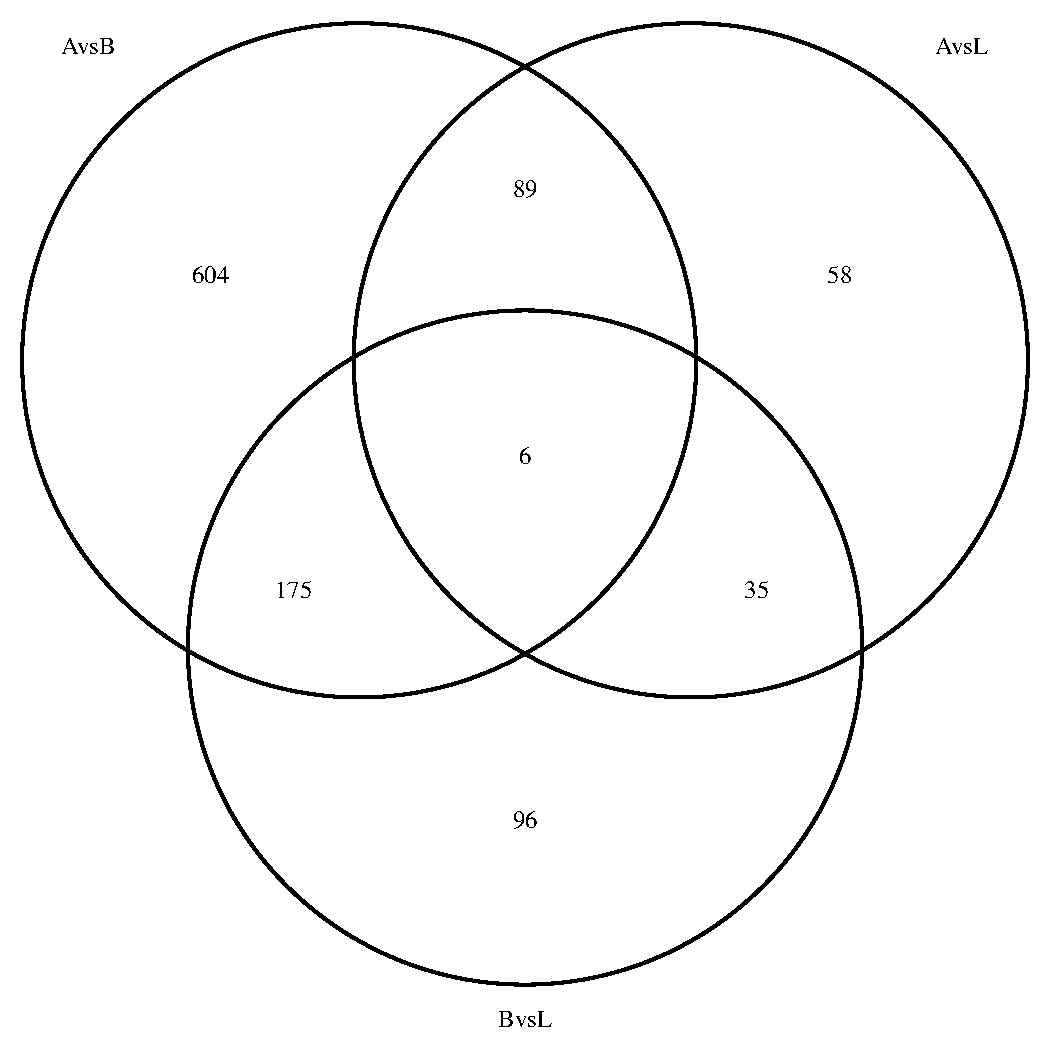
\includegraphics[width=\maxwidth]{images/graficvennSigGenes2-1} 
\begin{kframe}\begin{verbatim}
## null device 
##           1
\end{verbatim}
\end{kframe}
\end{knitrout}

\section{Analysis methods and tools}

Following \cite{Khatri:2012} three different approaches can be applied on these data:
\begin{itemize}
  \item \textbf{Classical enrichment or Overrepresentation Analysis}. This has been done using ad-hoc functions included in our analysis pipelines and also using DAVID a public software tool available at \url{https://david.ncifcrf.gov/}.
  \item \textbf{Gene Set Expression Analysis}. This can be done using the Bioconductor package \texttt{gage} which provides nice representations of genes overexpressed/downregulated in the context of KEGG pathways. A simpler but powerful version of this type of analysis can be applied with package \texttt{GSA}.
  \item A \textbf{Network analysis} can be done using Bioconductor packages such as \texttt{FGNet}. It is also possible to use commercial software such as the Ingenuity Pathways Software.
\end{itemize}

\subsection{Enrichment Analysis with \texttt{GOstats} and \texttt{DAVID}}

Given a list of (potentially) differentially expressed genes Enrichment Analysis or Overrepresentation Analysis (\textbf{ORA}) seeks to select functions and biological processes that characterize this list, this meaning that these functions appear more often in the list than in the remaining set of analyzed genes.

There have been developped many variations of this type of analysis (\cite {Khatri:2005}). 
We have applied ``classical'' enrichment analysis (\cite{Gentleman:2004}) implemented in the \texttt {GOstats} and \texttt{topGO} Bioconductor packages. We also present the improved version of ORA implemented in the DAVID software package, which is powerful but harder to use because it is based on an online tool difficult to "script".

\subsubsection{Enrichment Analysis using \texttt{GOstats}}

\subsubsection{Enrichment Analysis using \texttt{topGO}}

\subsubsection{Enrichment Analysis (?) using DAVID}

DAVID (the Database for Annotation, Visualization and Integrated Discovery, \cite{DAVID:2009}) is a free online bioinformatics resource developed by the Laboratory of Immunopathogenesis and Bioinformatics at NIH (\emph{National Institute of Allergy and Infectious Diseases (NIAID)}). 

DAVID provides a set of tools to help the functional interpretation of lists of genes derived from genomic studies. DAVID can be found at \url{http://david.niaid.nih.gov} or \url{http://david.abcc.ncifcrf.gov}

Given an uploaded gene list, the DAVID Resources provides classical gene-term enrichment analysis, but also new tools and functions that allow users to condense large gene lists into gene functional groups or cluster redundant and heterogeneous terms into groups. This grouping jointly with the dynamical access from results to Biological knowledge database provides a clearer and easy to interpret output than classical enrichment analysis.

\subsection{Gene Set Enrichment Analysis}

Gene set analysis (GSA) is a widely used strategy for gene expression data analysis based on pathway knowledge. GSA focuses on sets of related genes and has established major advantages over individual gene analyses, including greater robustness, sensitivity and biological relevance. 

\subsubsection{Gene Set Enrichment Analysis with \texttt{GAGE}}

We have applied a recent version of GSA called Generally Applicable Gene-set Enrichment (GAGE, \cite{GAGE:2009}). This method is more robust than other existing related approaches and has been seen to work well with different sample sizes, experimental designs and profiling techniques. GAGE has been shown to provide significantly good results results in the following three aspects: (1) consistency across repeated studies/experiments; (2) sensitivity and specificity; (3) biological relevance of the regulatory mechanisms inferred.

Essentially what GAGE -as most GSEA methods- does is to test if a given gene set is \emph{associated} with a gene list. That is for each gene set tested it selects those gene sets whose expression tends to be higher or lower than the expression of the genes in the genelist (in which case the gene set is called to be upregulated or downregulated).

Gene Sets can be GO categories or KEGG pathways and each is shown in a different format.
\begin{itemize}
  \item GO categories over or underrepresented are shown in a heatmap
  \item KEGG pathways are shown on a picture of the pathway with the genes that belong to the list marked in red or green depending on if they are up or down-regulated.
\end{itemize}

\subsubsection{Gene Set Enrichment Analysis with \texttt{GSA}}

The \texttt{GSA} package offers a simple approach to gene set analysis which has two main advantages:
\begin{itemize}
  \item It is very intuitive and simple to use
  \item It can be applied in situations more complex than the usual "two sample test" that many GSEA methods assume.
\end{itemize}
An obvious drawback is that the output is also simple and consists of a list of differentially expressed gene sets, without any links to databases or pathway visualizations.

\subsection{Network Analysis}

Network analysis is a generic expression to describe distinct analysis that use some type of network or graph representation of the data or the results. Related with what we are describing here one can find different methods for \emph{Module enrichment analysis} aimig at finding subnetworks with a particular biological meaning. We consider two such programs here, \texttt{FGNet} and \texttt{Inegnuity Pathway Analysis}.

\subsubsection{Analysis with \texttt{FGNet}}

\subsubsection{Analysis with \texttt{IPA}}

Ingenuity Pathway Analysis is a commercial tool allows searching and using information extracted from public databases and from full text article extraction. It categorizes its findings based on a in-house curated ontology, covering entities (proteins and other molecules), relationships between the entities (inhibites, activates,...) and functional information (pathways, biological process, disease,...).

IPA has several differences with the previous tools.
\begin{itemize}
  \item It relies not only on public databases but on their own commercial databases and ontology, that they claim to be better anotated and more intuitive.
  \item It performs enrichment analysis but besides it does different types of network analysis and allows to view selected genes in:
  \begin{enumerate}
  \item Association networks, based on co-citation of genes in the literature
  \item Canonical pathways based on known biological pathways.
\end{enumerate}
\item It provides other types of information for analyzed genes such as their association with disease or their potential toxicogenomic properties.
\end{itemize}

\section{Results}

This section contains the results of applying \emph{some of} the analyses described above to the examples lists.

\subsection{Gene enrichment analysis using \texttt{GOstats}}

We present below two ways to do enrichment analysis with GOStats.
The first one makes direct use of functions available in the \texttt{GOstats} package, while the second uses some home-encapsulated functions.

\begin{knitrout}
\definecolor{shadecolor}{rgb}{0.969, 0.969, 0.969}\color{fgcolor}\begin{kframe}
\begin{verbatim}
## 
## Comparison:  AvsB 
## GO
##       GOBPID       Pvalue OddsRatio  ExpCount Count Size
## 1 GO:0006629 2.588340e-06  1.707120 79.057118   117  567
## 2 GO:0044255 1.034654e-05  1.744666 61.210009    93  439
## 3 GO:0032787 1.275704e-05  1.985539 35.973080    61  258
## 4 GO:0008610 2.121849e-05  1.891353 40.434858    66  290
## 5 GO:0002682 2.469534e-05  1.551362 99.971700   137  717
## 6 GO:0007259 3.052054e-05  3.385397  8.365833    21   60
##                                    Term
## 1               lipid metabolic process
## 2      cellular lipid metabolic process
## 3 monocarboxylic acid metabolic process
## 4            lipid biosynthetic process
## 5   regulation of immune system process
## 6                      JAK-STAT cascade
## KEGG
##   KEGGID       Pvalue OddsRatio  ExpCount Count Size
## 1  05213 0.0003981226  3.901831  4.820961    13   33
## 2  05223 0.0008045551  3.782377  4.528781    12   31
## 3  04010 0.0024236800  2.001661 16.508138    28  113
## 4  03320 0.0024503737  2.992958  5.697499    13   39
## 5  04914 0.0054220691  2.538264  6.866217    14   47
## 6  01040 0.0064550128  5.076559  1.899166     6   13
##                                      Term
## 1                      Endometrial cancer
## 2              Non-small cell lung cancer
## 3                  MAPK signaling pathway
## 4                  PPAR signaling pathway
## 5 Progesterone-mediated oocyte maturation
## 6 Biosynthesis of unsaturated fatty acids
## 
## Comparison:  AvsL 
## GO
##       GOBPID       Pvalue OddsRatio   ExpCount Count Size
## 1 GO:0044281 5.440527e-06  2.111702 36.6372735    62 1173
## 2 GO:0005996 4.001358e-05  3.811863  4.5289042    15  145
## 3 GO:0044282 5.275232e-05  3.532283  5.1848145    16  166
## 4 GO:0006570 1.171659e-04 94.601124  0.1249353     3    4
## 5 GO:0043436 1.678394e-04  2.216064 16.4914582    32  528
## 6 GO:0006082 1.931328e-04  2.196617 16.6163934    32  532
##                               Term
## 1 small molecule metabolic process
## 2 monosaccharide metabolic process
## 3 small molecule catabolic process
## 4       tyrosine metabolic process
## 5        oxoacid metabolic process
## 6   organic acid metabolic process
## KEGG
##   KEGGID       Pvalue OddsRatio   ExpCount Count Size
## 1  00983 0.0002266541 12.047952  0.6097658     5   16
## 2  00350 0.0005507651  9.454474  0.7240969     5   19
## 3  01100 0.0017676527  1.982550 21.3036919    34  559
## 4  00360 0.0038130654 12.994624  0.3429933     3    9
## 5  00010 0.0055977524  5.065511  1.1814212     5   31
## 6  00982 0.0071986206  6.153453  0.8003176     4   21
##                                Term
## 1   Drug metabolism - other enzymes
## 2               Tyrosine metabolism
## 3                Metabolic pathways
## 4          Phenylalanine metabolism
## 5      Glycolysis / Gluconeogenesis
## 6 Drug metabolism - cytochrome P450
## 
## Comparison:  BvsL 
## GO
##       GOBPID       Pvalue OddsRatio    ExpCount Count Size
## 1 GO:0036499 9.461963e-06 19.802158   0.5880932     6   12
## 2 GO:0032501 1.017167e-05  1.694021 121.6372735   157 2482
## 3 GO:0044707 1.104044e-05  1.690072 118.8438309   154 2425
## 4 GO:0006984 1.571641e-05  9.367434   1.2251941     8   25
## 5 GO:0048732 2.050040e-05  2.776800  10.7327006    26  219
## 6 GO:0008285 2.216348e-05  2.404664  16.1235548    34  329
##                                        Term
## 1   PERK-mediated unfolded protein response
## 2          multicellular organismal process
## 3     single-multicellular organism process
## 4              ER-nucleus signaling pathway
## 5                         gland development
## 6 negative regulation of cell proliferation
## KEGG
##   KEGGID       Pvalue OddsRatio ExpCount Count Size
## 1  05219 0.0006285001  5.871449 1.554188     7   29
## 2  05216 0.0033135057  6.074359 1.071854     5   20
## 3  00010 0.0051396857  4.388837 1.661374     6   31
## 4  05222 0.0070941074  3.201643 2.894006     8   54
## 5  04974 0.0094987904  3.777065 1.875744     6   35
##                               Term
## 1                   Bladder cancer
## 2                   Thyroid cancer
## 3     Glycolysis / Gluconeogenesis
## 4           Small cell lung cancer
## 5 Protein digestion and absorption
\end{verbatim}


{\ttfamily\noindent\bfseries\color{errorcolor}{\#\# Error in `*tmp*`[[i]]: subscript out of bounds}}\end{kframe}
\end{knitrout}

The analysis below is done using the functions defined in file \texttt{hyperGeometricAnalysis.R}



\subsection{Gene enrichment analysis using \texttt{topGO}}

The analysis using \texttt{topGO} is relatively similar to the one done with \texttt{GOstats}. One creates a data structure that is used to call the main analysis function. However it is different from that from \texttt{GOstats} in that, instead of two lists of genes (Universe/Differentially expressed) it is provided with a list of scores, \emph{whose names are the gene names} and the name of a function whos output (TRUE/FALSE) helps selecting which genes are differentially expressed in the list.

Warning: We are using the \texttt{R2HTML} package to write the output. This package doesn't admit whitespaces in the output path so files are written to another directory and recovered later.

\begin{knitrout}
\definecolor{shadecolor}{rgb}{0.969, 0.969, 0.969}\color{fgcolor}\begin{kframe}


{\ttfamily\noindent\itshape\color{messagecolor}{\#\# Loading required package: R2HTML}}\begin{verbatim}
## 
## Building most specific GOs .....
\end{verbatim}


{\ttfamily\noindent\itshape\color{messagecolor}{\#\# Loading required package: hgu133a.db}}

{\ttfamily\noindent\itshape\color{messagecolor}{\#\# }}\begin{verbatim}
## 	( 8208 GO terms found. )
## 
## Build GO DAG topology ..........	( 12028 GO terms and 28831 relations. )
## 
## Annotating nodes ...............	( 5795 genes annotated to the GO terms. )
## 
## 			 -- Classic Algorithm -- 
## 
## 		 the algorithm is scoring 4249 nontrivial nodes
## 		 parameters: 
## 			 test statistic:  fisher 
## 
##  *** Output redirected to directory:  ~
##  *** Use HTMLStop() to end redirection.
## Building most specific GOs .....	( 8208 GO terms found. )
## 
## Build GO DAG topology ..........	( 12028 GO terms and 28831 relations. )
## 
## Annotating nodes ...............	( 5795 genes annotated to the GO terms. )
## 
## 			 -- Classic Algorithm -- 
## 
## 		 the algorithm is scoring 4073 nontrivial nodes
## 		 parameters: 
## 			 test statistic:  fisher 
## 
##  *** Output redirected to directory:  ~
##  *** Use HTMLStop() to end redirection.
## Building most specific GOs .....	( 8208 GO terms found. )
## 
## Build GO DAG topology ..........	( 12028 GO terms and 28831 relations. )
## 
## Annotating nodes ...............	( 5795 genes annotated to the GO terms. )
## 
## 			 -- Classic Algorithm -- 
## 
## 		 the algorithm is scoring 4183 nontrivial nodes
## 		 parameters: 
## 			 test statistic:  fisher 
## 
##  *** Output redirected to directory:  ~
##  *** Use HTMLStop() to end redirection.
\end{verbatim}
\end{kframe}
\end{knitrout}

With \texttt{topGO} it is possible to extract a graph with nodes colored according to the significance. Below is shown the graph associated with the first comparison. Additionally all graphs are written to .pdf files

\begin{knitrout}
\definecolor{shadecolor}{rgb}{0.969, 0.969, 0.969}\color{fgcolor}
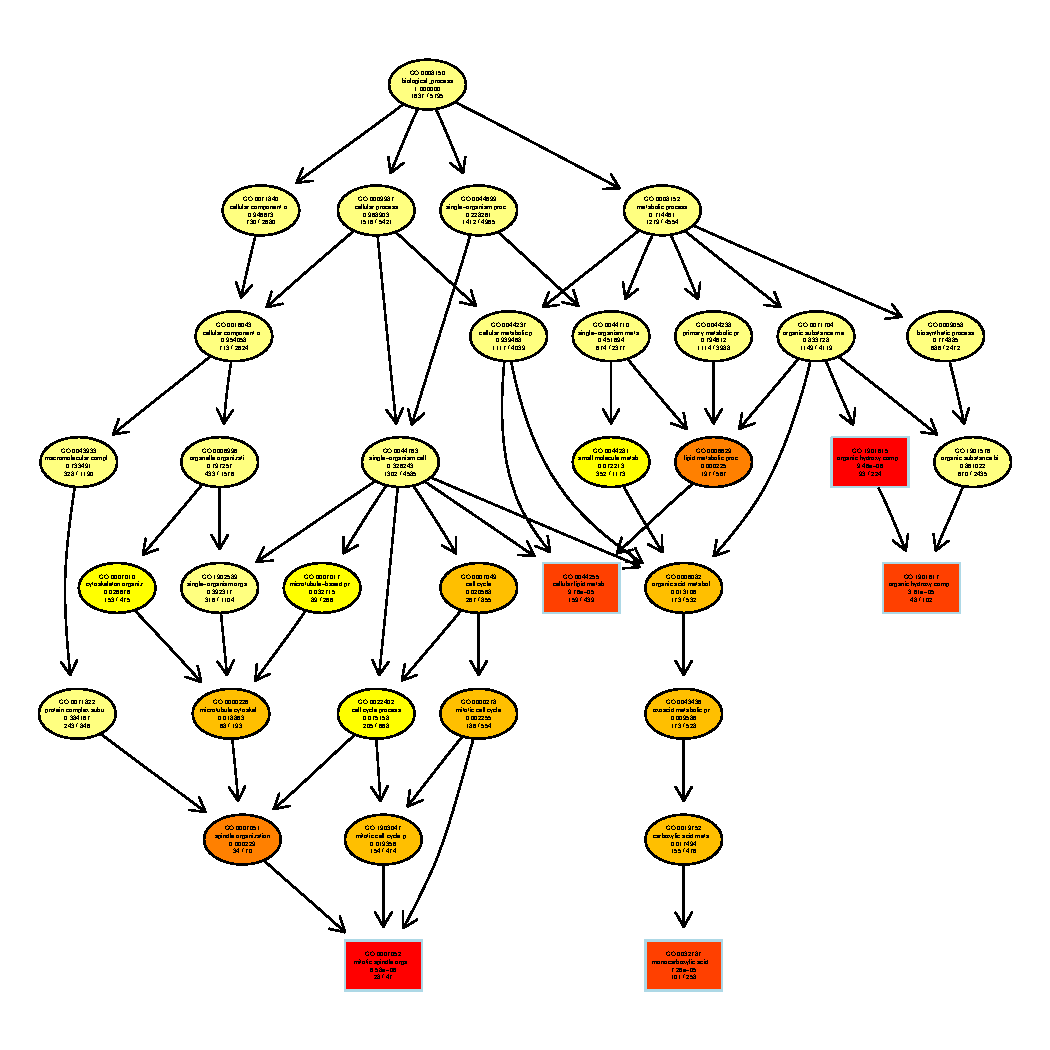
\includegraphics[width=\maxwidth]{images/graficGOgraphs-1} 
\begin{kframe}\begin{verbatim}
## $dag
## A graphNEL graph with directed edges
## Number of Nodes = 35 
## Number of Edges = 56 
## 
## $complete.dag
## [1] "A graph with 35 nodes."
\end{verbatim}
\end{kframe}
\end{knitrout}

\subsubsection{Comparison between \texttt{GOstats} and \texttt{topGO} output}

\section{Results presentation}

The results of the analyses performed following the methodology described in the previous sections consist  of a  high number of tables and figures.

In order to facilitate its organization and review a web page (an html file indeed) is prepared that allows to access each file.

This page consists consists of a list of links organized by topics which correspond to the files outputted as result of the different steps undertaken in the analysis.

A brief description of each group of results and its contents follows below.

\begin{enumerate}
 \item Section \textbf{Reports and results summaries} gives access to the report describing the goals and methods applied in the analysis.
\item Section \textbf{Input Files for Biological Significance} gives access to different files from where the genes to be included in the analysis have been obtained.
\item Section \textbf{Gene Set Expression Analysis (GAGE)} gives access to the lists of results found, for each comparison of interest, in the Gene Set Enrichment Analysis against the Kyoto Encyclopedia of Genes and the Gene Ontology database, considering up- and down-regulated elements separately. 
\begin{itemize}
\item For the analysis against the Gene Ontology database. GO Molecular Functions (MFs), GO Biological Processes (BPs), and GO Cellular Components (CCs) classifications have been tested, considering up- and down-regulated elements separately. In this case, only GO terms with an enrichment test q-value (adjusted p-value) below 0.05 have been considered as relevant and included in the tables.
\item For each KEGG analyis, a zipped folder with details (plots and xml or txt files) is provided. In this case, only pathways with an enrichment test q-value (adjusted p-value) below 0.15 have been considered as relevant and included in the tables.
\end{itemize}

\item Section \textbf{DAVID Analysis Results}

This section gives access to two types of files generated by DAVID
\begin{itemize}
  \item Functional annotation chart with the main results of enrichment analysis
  \item Functional annotation clustering where the resulting categories obtained from enrichment analysis are grouped by similarity of functions.
\end{itemize}


\item Section \textbf{Ingenuity Pathway Analysis}

IPA generates many types of results and is intended to be used interactively exploring them on their web site (which requires a password protected access). In order to have an overview of what has been obtaineda pdf with a summary of these resuts can be generated.

The links in this section give access to the analysis summary for each gene list.

\end{enumerate}



\bibliography{MDAreferences}

\end{document}

%%%%%%%%%%%%%%%%%%% Old code




